\subsection{Quantum Random Walks}
Quantum random walks, as mentioned in section \ref{section:intro}, are a model for universal quantum computation, meaning that any computation that is possible for a quantum computer can be simulated by a QW.
Like much of quantum computing, QWs can be motivated from a classical predecessor, the \emph{classical random walk}.
Here the classical random walk is used specifically to motivate the discrete QW since the protocol presented in section \ref{section:qw_transfer} makes use of such a QW.
Hence all future references to QWs are assumed to be of the discrete variant.

\subsubsection{Motivation from the Classical Random Walk}
\label{subsubsection:classc_r_w}
In the classical random walk, a walker is constrained to moving up and down a discrete number line, starting their walk at the origin.
To determine whether to take a step to the left (-1) or the right (+1), the walker flips an unbiased coin, moving to the right if the coin lands on heads and to the left if the coin lands on tails. 
This process of flipping a coin and taking a step can be repeated until a desired stopping point is reached, e.g. after a given number of coin flips.
The walk can also continue on forever and in this limit, the walker will reach every point on the number line.
In this report, however, only finite length walks are considered.
Without much thought it can be concluded that after $T$ coin flips the walker can be at most $\pm T$ steps away from the origin, corresponding to the case where every step taken is in the same direction.
The probability distribution describing the probability of the walker being in any given position away from the origin is given by a binomial distribution, an example of which is shown in orange in figure \ref{fig:discVSclass} for 100 coin flips.

\subsubsection{Quantum Walk on a Line}
\label{subsubsection:q_r_w}
Having described the classical random walk, it can now be "quantised" into the \emph{quantum random walk}.
The QW is considered as a composite system of the coin, belonging to the Hilbert space $\mathcal{H}_C$ and walker, $\mathcal{H}_C$,
\begin{equation}
    \mathcal{H} = \mathcal{H}_C \otimes \mathcal{H}_W.
\end{equation}
Note that this use of subscript does not depart from the earlier usage to indicate the dimension of the Hilbert space, since the $\mathcal{H}_C$ is spanned by two states (the "heads" state and the "tails" state), and $\mathcal{H}_W$ is spanned by all the points on the number line to be walked upon, so can be thought of as an unspecified $d$ dimensional space.
Therefore the labels $C$ and $W$, also serve to indicate the dimension of the labelled space.

To aid distinguishability between coin states and position states, they are labelled by
\begin{align}
    \langle\mathcal{H}_C\rangle &= \{\ket{\uparrow}, \ket{\downarrow}\}\\
    \langle\mathcal{H}_W\rangle &= \{\ket{k} | -T\leq k \leq +T, k\in\mathbb{Z}\},
\end{align}
where $\langle U \rangle$ denotes a set of states which span $U$, and $T$ again is the number of "coin flips".
Therefore, the states $\ket{\uparrow}, \ket{\downarrow}$ take the place of heads and tails on our quantum "coin". 
Note in particular that there is no constraint placed on the dimensionality of $\mathcal{H}_W$, and therefore the walker can be taken to be a qudit, whereas $\dim{\mathcal{H}_C} = 2$ and the coin is taken to be a qubit.
Now that the Hilbert space of the system has been contructed, operators are required in order for the system to evolve.
In the classical random walk, the first operation needed was a coin flip so in similar fashion the quantum walk too needs a coin flip operator, $C\in \mathcal{H}_C$ (not to be confused with the $\C{U}$ controlled-unitary operator).
There is a continuum of choices for $C$, and indeed QWs can be constructed on a whole host of different graphs - see for a greater discussion \cite{Tregenna2003}. 
For walks on a line, constraining the coin to have real coefficients leaves the Hadamard coin as the only choice of coin available.
This takes on the same form as the Hadamard transform defined in section \ref{subsection:qc_primer} and is given here via an alternative expression,
\begin{align}
    H &= \frac{1}{\sqrt{2}}\Big[
    \ket{\uparrow}\bra{\uparrow} +
    \ket{\uparrow}\bra{\downarrow} +
    \ket{\downarrow}\bra{\uparrow} -
    \ket{\downarrow}\bra{\downarrow}\Big]\\
    &= \frac{1}{\sqrt{2}}\Big[(\ket{\uparrow} + \ket{\downarrow})\bra{\uparrow} +
    (\ket{\uparrow} - \ket{\downarrow})\bra{\downarrow}\Big]
    \label{equation:hadamard_coin}
\end{align}
where $\ket{0} \rightarrow \ket{\uparrow}$ and $\ket{1} \rightarrow \ket{\downarrow}$.
As before, if the coin state is $\ket{\uparrow}$ then it becomes an equal superposition of $\ket{\uparrow} + \ket{\downarrow}$, if the coin state is in $\ket{\downarrow}$ then we get an equal superposition of $\ket{\uparrow} - \ket{\downarrow}$ and this is made particularly clear by equation \ref{equation:hadamard_coin}.
Following this, a shift operator $S \in \mathcal{H}$ is needed to move the walker dependent on the state of the coin.
\begin{equation}
    S = \sum_k \ket{\uparrow}\bra{\uparrow} \otimes \ket{k + 1}\bra{k} + \ket{\downarrow}\bra{\downarrow} \otimes \ket{k - 1}\bra{k}.
\end{equation}
Again, representing $S$ in this way makes manifest its effect on the walker. 
If the coin state is $\ket{\uparrow}$, the walker takes a step in the +1 direction, if it is $\ket{\downarrow}$ then a step in the -1 direction is taken.
The probability distribution of such a walk is plotted in blue in fig \ref{fig:discVSclass}, where the initial coin state is $\ket{\downarrow}$, and is compared to a classical random walk.\newline

\begin{figure}
    \centering
    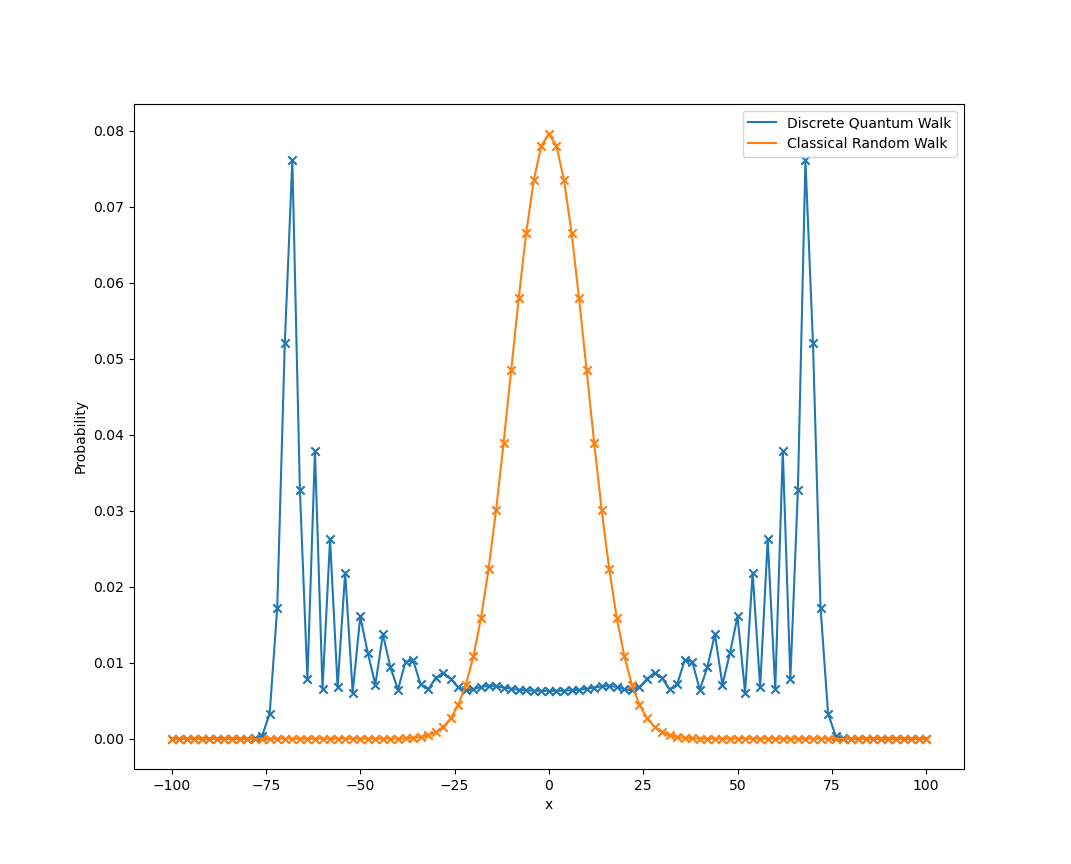
\includegraphics[scale=0.75]{Discrete vs Classical Walk.png}
    \caption{The probability distributions of a classical and Hadamard-coined quantum walk on a line, both originating at the origin. The quantum walk coin is initially in the $\frac{1}{\sqrt{2}}\left(\ket{\uparrow} + i\ket{\downarrow}\right)$ state. Odd points have been omitted as they all have zero probability.}
    \label{fig:discVSclass}
\end{figure}

Whilst the above choice of $S$ is the most common on the number line, there are alternatives such as
\begin{equation}
    \tilde{S} = \sum_k \ket{\uparrow}\bra{\uparrow} \otimes \ket{k}\bra{k} + \ket{\downarrow}\bra{\downarrow} \otimes \ket{k + 1}\bra{k}.
\end{equation}
Th subtle difference between $\tilde{S}$ and $S$ is that $\tilde{S}$ can only move in the $+1$ direction of the number line and has no "left moving" part.
This means that $\tilde{S}$ is restricted to the non-negative integers and unlike $S$, can occupy all $\ket{x}$ for $0\leq x\leq T$, where $T$ is the number of time steps in our QW.
In fact $\tilde{S}$ is an operator that was introduced earlier in section \ref{subsubsection:operators},
\begin{equation}
    \tilde{S} = \C{X}.
\end{equation}
\FloatBarrier